\section{Introduction}
\label{sec:introduction}

\indent

% state the learning objective 
The objective of this laboratory assignment is to study an audio amplifier.
This circuit is made up of a gain stage and an output stage.
The format of the circuit can be seen in Figure~\ref{fig:format}. And the  provided circuit can be seen in Figure~\ref{fig:circuit}.

In Section~\ref{sec:theoretical analysis}, a theoretical analysis of the circuit is
presented. In Section~\ref{sec:simulation analysis}, the circuit is analysed by
means of a ngspice simulation. The results are then compared to the theoretical results obtained in
Section~\ref{sec:theoretical analysis}. The conclusions of this study are outlined in
Section~\ref{sec:conclusion}.



\begin{figure}[h!] \centering
	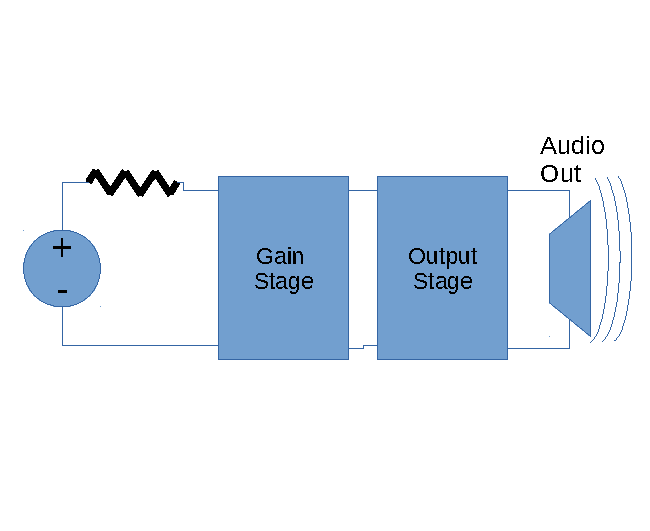
\includegraphics[width=0.65\linewidth]{circ_enunciado.pdf}
	\caption{Assigned Circuit.}
	\label{fig:format}
\end{figure}

\begin{figure}[h!] \centering
	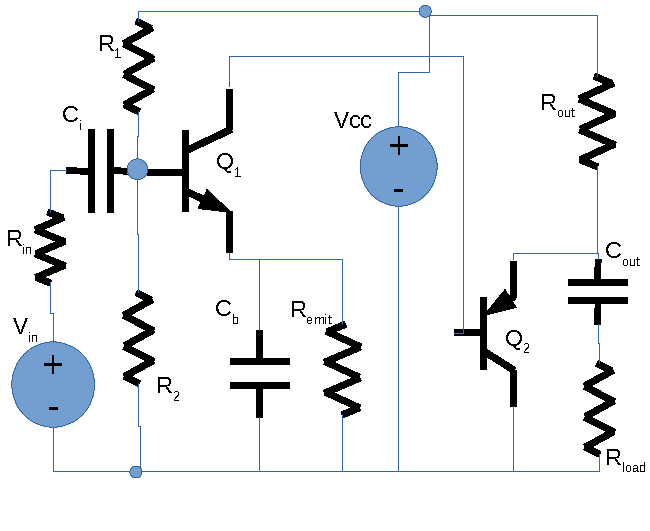
\includegraphics[width=0.6\linewidth]{circ.pdf}
	\caption{Chosen Circuit.}
	\label{fig:circuit}
\end{figure}



